% -*- mode: fundamental -*-

% Slides accompanying "Learn RISC-V CPU Implementation and BSV" book
% Copyright (c) 2024 Rishiyur S. Nikhil, All Rights Reserved

% -*- mode: fundamental -*-

% Slides accompanying "Learn RISC-V CPU Implementation and BSV" book
% Copyright (c) 2024 Rishiyur S. Nikhil, All Rights Reserved

% This is a preamble shared by all the slide decks

\documentclass[10pt, aspectratio=169]{beamer}

% \documentclass[17pt]{beamer}

% Avail. font sizes: 8pt, 9pt, 10pt, 11pt, 12pt, 14pt, 17pt, 20pt.
% Default font size is 11pt (= 22pt in full screen mode).

\usepackage{verbatim}
\usepackage{fancyvrb}
\usepackage{listings}

% ================================================================
% Themes

\usetheme{Madrid}          % Line at bottom: Author (affiliation), OptTitle, Conf, page 

% \usetheme{Copenhagen}    % Same as Madrid except bottom line: Author, OptTitle

% \usetheme{Berkeley}    % Takes up 1-inch border on left and top

% ----------------
% colorthemes
% (default), beaver, beetle, seahorse, wolverine

\usecolortheme{seahorse}

% ================================================================
% Customization: show table of contents before each section
% Use \AtBeginSubsection    to show before each subsection

% \AtBeginSection[]
% {
%   \begin{frame}
%     \frametitle{Table of Contents}
%     \tableofcontents[currentsection]
%   \end{frame}
% }

% ================================================================

% ----------------
% The bsc compiler and BSV language
\newcommand{\bsc}{\emph{bsc}}
\newcommand{\BSV}{\bf{BSV}}
% ----------------
% ITALICISE WORDS
\newcommand{\ie}{\emph{i.e.,}}
\newcommand{\eg}{\emph{e.g.,}}
\newcommand{\Eg}{\emph{E.g.,}}
\newcommand{\etc}{\emph{etc.}}
\newcommand{\via}{\emph{via}}
\newcommand{\vs}{\emph{vs.}}

% ----------------
% EMPTY BOXES OF VARIOUS WIDTHS, FOR INDENTATION

\newcommand{\hm}{\hspace*{1em}}
\newcommand{\hmm}{\hspace*{2em}}
\newcommand{\hmmm}{\hspace*{3em}}
\newcommand{\hmmmm}{\hspace*{4em}}

% ----------------
% Convenient widths

\newlength{\hlessmm}
\setlength{\hlessmm}{\textwidth}
\addtolength{\hlessmm}{-2em}

\newlength{\hlessmmm}
\setlength{\hlessmmm}{\textwidth}
\addtolength{\hlessmmm}{-3em}

\newlength{\hlessmmmm}
\setlength{\hlessmmmm}{\textwidth}
\addtolength{\hlessmmmm}{-4em}

% ================================================================
% Title page

\title[Learn CPU design \& BSV]{Learn RISC-V CPU Implementation and BSV}

\subtitle{(BSV: a High-Level Hardware Design Language)}

\author[{\copyright} R.S.Nikhil]{Rishiyur S.~Nikhil}
% \institute{Bluespec, Inc.}

% Date is set differently in each slide deck

% \logo{
\includegraphics[height=0.6cm]{../Figures/Bluespec_Logo_2022-10}}

% End of preamble
% ****************************************************************


\date{L1: Introduction}

% ****************************************************************

\begin{document}

% ================================================================

\begin{frame}
 \titlepage

 \begin{center}
  
\includegraphics[height=1cm]{Bluespec_Logo_2022-10}
 \end{center}
\end{frame}


% ****************************************************************

\begin{frame}
\frametitle{Goals for this book/course}

\footnotesize

\begin{center}
 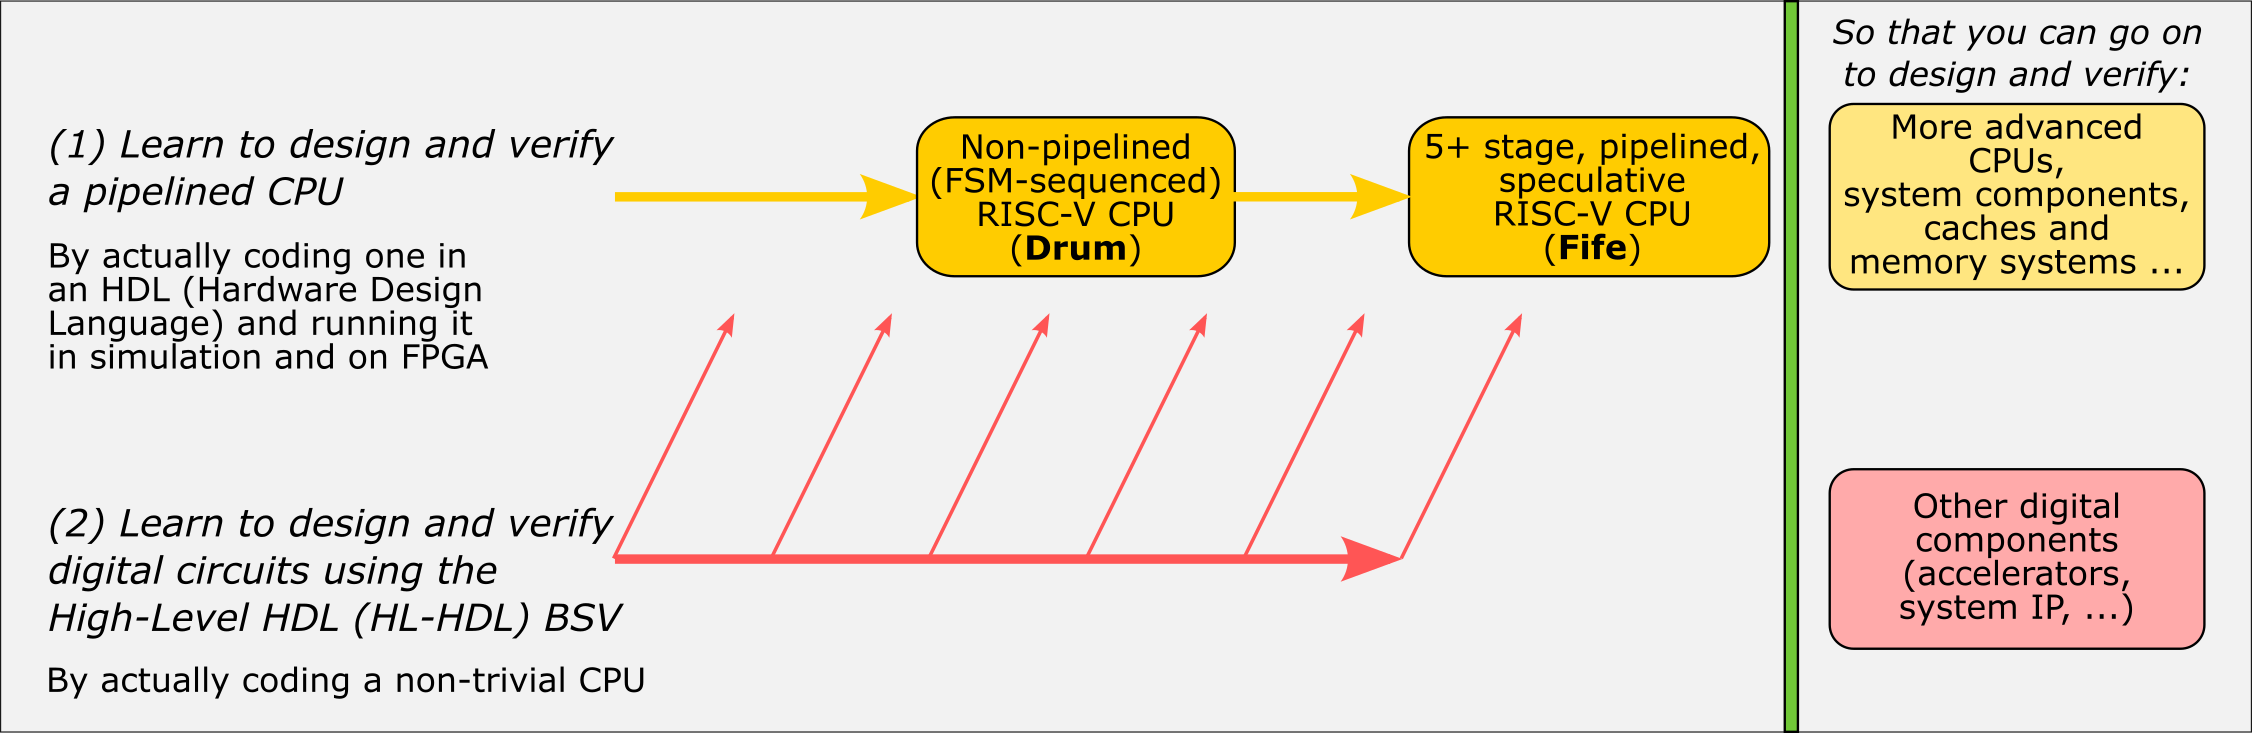
\includegraphics[width=0.9\textwidth]{Fig_Goals}
\end{center}

These goals are complementary:
\begin{itemize}

 \item One cannot really learn CPU design without actually doing it,
       for which we need an HDL.

 \item One cannot really learn an HDL without actually doing it, for
       which we need interesting examples.

\end{itemize}

\end{frame}

% ****************************************************************

\begin{frame}
\frametitle{Learn {\BSV} to design the CPUs}

\footnotesize

\begin{itemize}

 \item {\BSV} is a high-level hardware design language (HL-HDL).

 \item Modern (features on par with modern software programming languages).

 \item Industrial strength; stable language and tools.

       More than 20 years usage in industry and academia for major hardware designs.
\end{itemize}

\end{frame}

% ================================================================

\begin{frame}
\frametitle{Topics we will cover (in red text)}

\footnotesize

\begin{center}
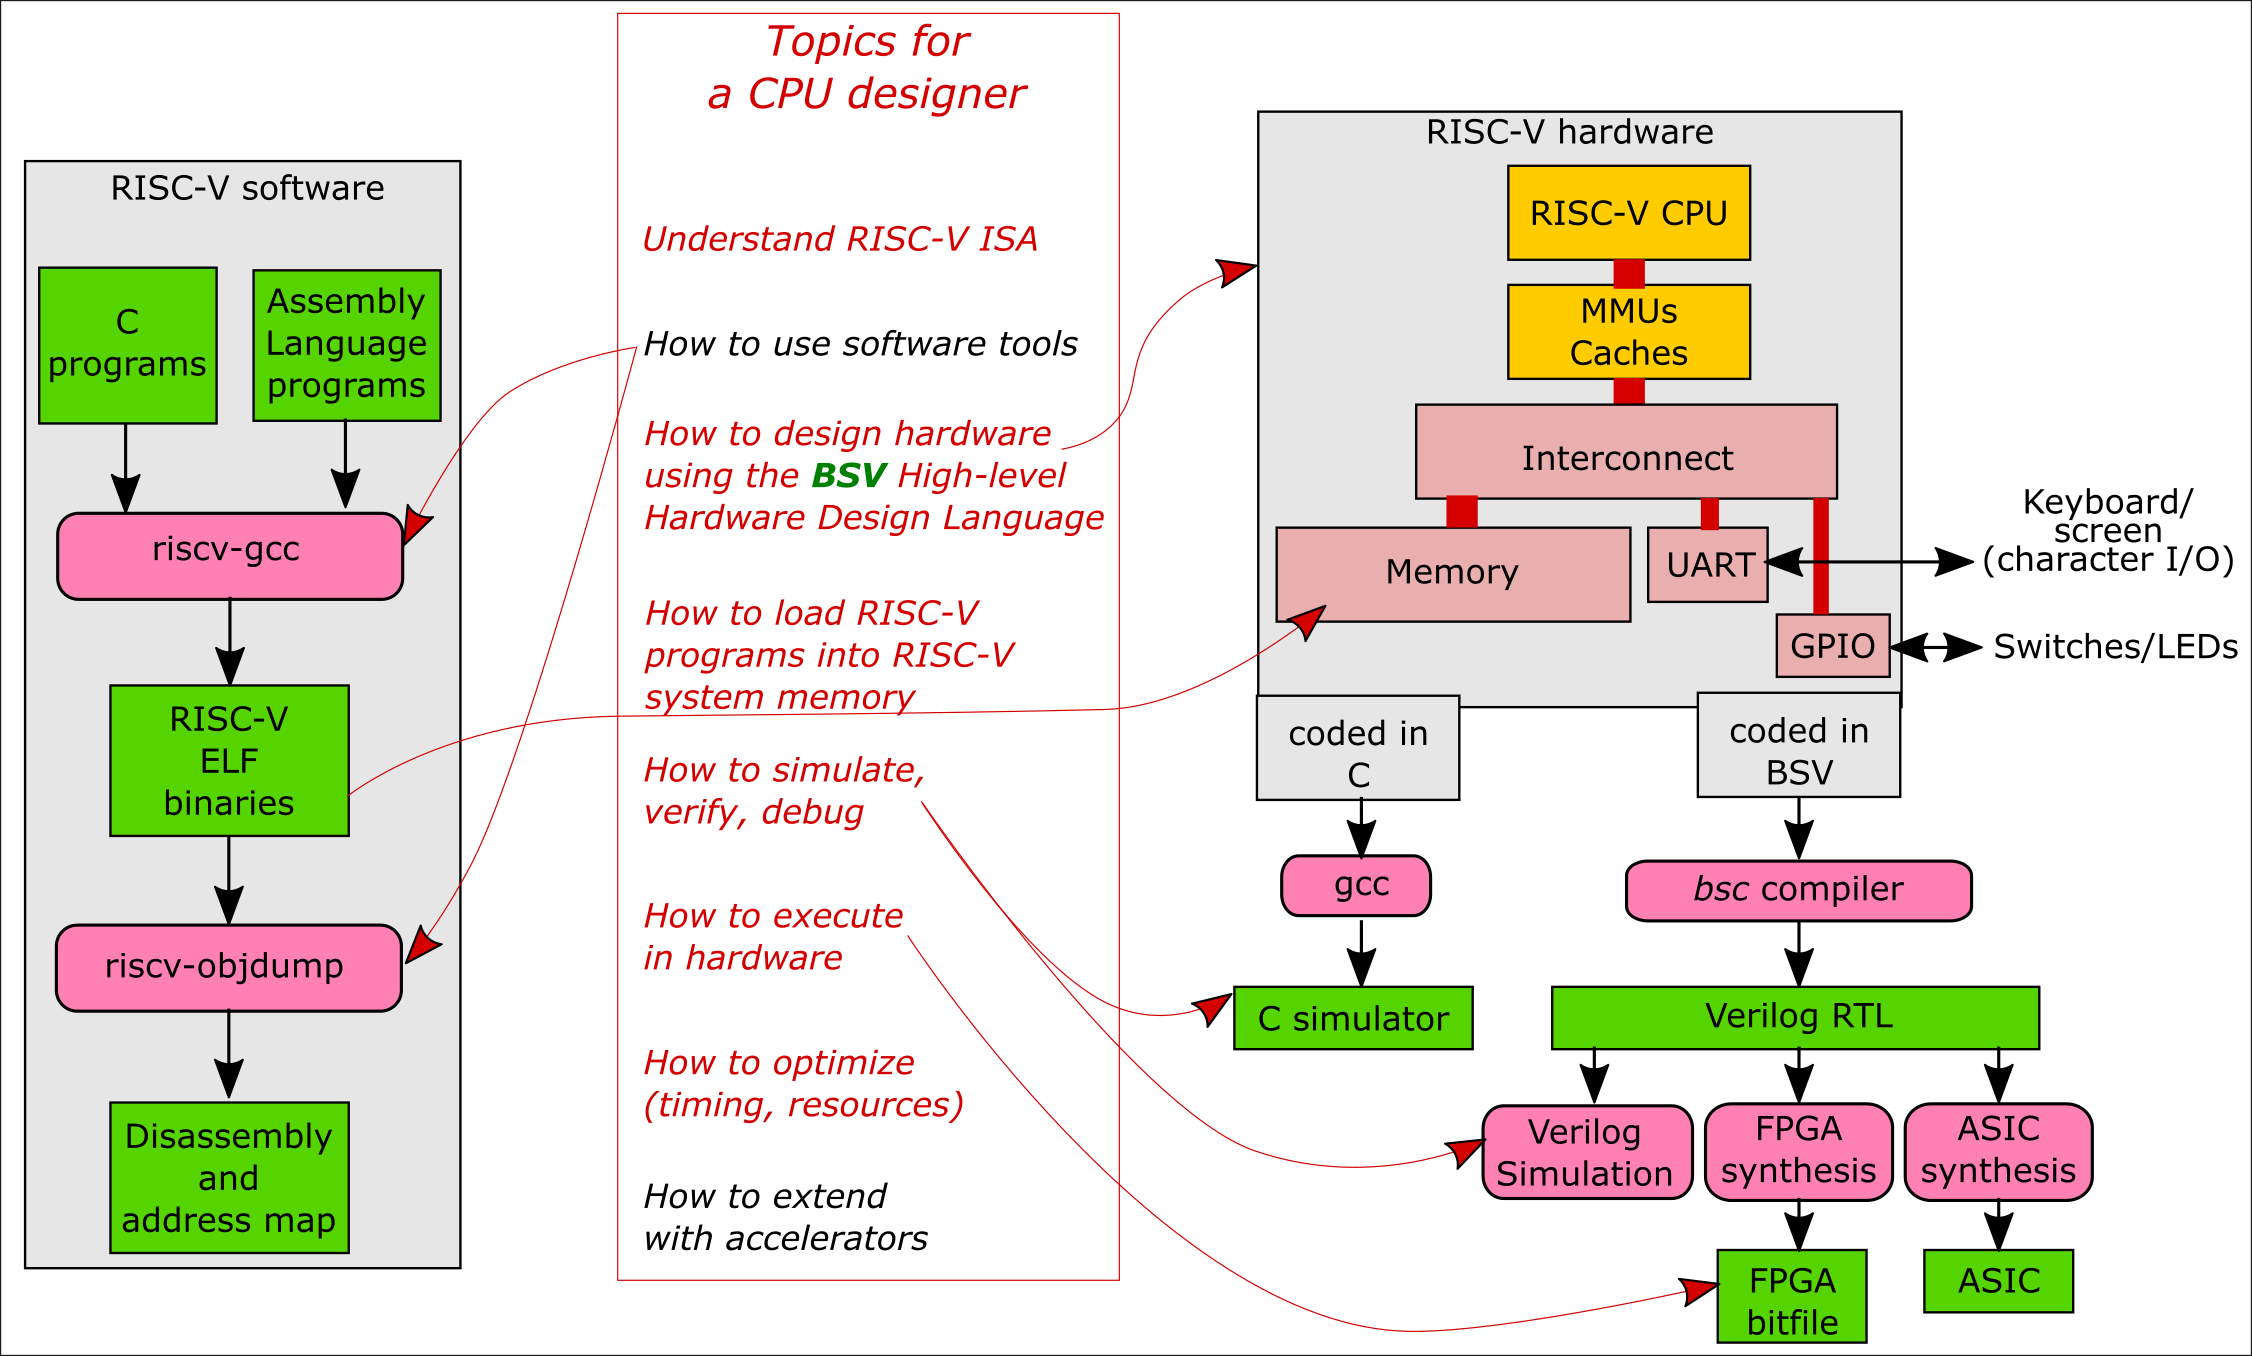
\includegraphics[height=0.8\textheight]{Fig_Topics}
\end{center}

\end{frame}

% ================================================================

\begin{frame}
\frametitle{Two CPU implementations (microarchitectures): Drum and Fife}

\footnotesize

\begin{center}
\frame{\includegraphics[width=0.8\textwidth]{Fig_Two_Microarchitectures}}
\end{center}

The two implementations share much code capturing RISC-V functionality

\end{frame}

% ================================================================

\begin{frame}
\frametitle{Why two microarchitectures?}

\footnotesize

\begin{itemize}

 \item \emph{Incremental learning:} we can master all the
       \emph{functional} aspects of RISC-V with Drum, and focus
       entirely on pipelining aspects with Fife.

 \PAUSE{}

 \item \emph{Functional debugging:} Bugs may be due to:
       \begin{itemize}\footnotesize
        \item[(A)] wrong implementation of RISC-V functionality ({\eg} address calculation)
        \item[(B)] wrong implementation of pipelining ({\eg} register read/write hazard)
       \end{itemize}

       \vspace{1ex}

       Drum allows us to debug all aspects of (A) in a simpler system
       (no complications due to pipelining).

       \vspace{1ex}
       All this carries over directly into Fife, so when debugging Fife, we can focus on (B).

       \vspace{1ex}
       Drum can be viewed as a \emph{synthesizable reference model}
       for Fife or other RISC-V CPUs.

 \PAUSE{}

 \item \emph{Both implementations are useful in different applications:}

   \begin{itemize}\footnotesize
   \item Drum uses smaller circuits (microcontrollers, embedded, IoT, ...)
   \item Fife is faster, larger, for more demanding applications
   \end{itemize}
\end{itemize}
\end{frame}

% ================================================================

\begin{frame}
\frametitle{Book and full source code; ready to build and execute}

\footnotesize

This course is based on:

\begin{itemize}
\item a free PDF textbook
\item full source code for Drum and Fife
  \begin{itemize}\footnotesize
  \item Free and open-source

  \item Drum and Fife CPU sources are written in {\BSV}.  Parts of the
        testbench are written in C.
  \end{itemize}
\end{itemize}

\PAUSE{\vspace{1ex}}

Use free and open-source tools to build Drum and Fife into
simulation executables, and have them execute RISC-V binaries
(ELF files, output of \emph{gcc}).

\begin{itemize}
\item {\BSV} code needs the \emph{bsc} compiler.

\item Two ways to simulate:
  \begin{itemize}\footnotesize
    \item Bluesim (standalone; just need \emph{bsc})
    \item Standard Verilog simulation \\
      We will demostrate using Verilator, but you can use any Verilog simulator.
  \end{itemize}
\end{itemize}

\PAUSE{\vspace{1ex}}

We will also demonstrate synthesis of Drum and Fife, and running on an FPGA. \\
(we will use an Amazon AWS ``F1 instance'', but you can use any FPGA).

\end{frame}

% ================================================================

\begin{frame}
\frametitle{Teaching methodology}

\footnotesize

Learn RISC-V CPU design and {\BSV} together:

\begin{itemize}
\item We will interleave RISC-V and {\BSV} topics, to learn them together.
\item We will learn a little {\BSV}, then apply that to some part of the RISC-V CPU design.
\item We will repeat this process until we have the full CPU designs.
\item Every example will involve actual {\BSV} code for Drum and/or Fife.
\end{itemize}

\PAUSE{\vspace{1ex}}

Learn Drum first, then Fife:

\begin{itemize}
\item We will learn all of Drum first, and have Drum execute RISC-V programs.
\item Then we will learn pipelining principles, and how we code them for Fife.
\item Fife executes the same RISC-V programs as Drum.
\end{itemize}

\PAUSE{\vspace{1ex}}

Debugging and optimization:

\begin{itemize}

\item Along the way we will develop testbenches for components and
      demonstrate debugging the {\BSV} code.

\item After Fife is running, we will discuss deeper optimizations for Drum and Fife.
\end{itemize}

\end{frame}

% ================================================================

\begin{frame}
\frametitle{Teaching methodology: an unconventional approach}

\footnotesize

Most courses on hardware design spend a lot of time on
circuit diagrams and schematics, boolean logic gates (AND, OR, NOT,
XOR, ...), combinational circuits, logic minimization, flip flops,
registers, binary number representations (twos complement), FSMs
(Finite State Machines), and so on.

\vspace{1ex}

However, most modern digital hardware design is done at a higher level
of abstraction.  Designs are described using languages like Verilog,
SystemVerilog and VHDL, and we rely on \emph{compilers} to produce
gates, wires, registers, {\etc}.  Accordingly, we will focus on
language-based hardware design, and not so much on the detailed
underlying circuits.

\vspace{1ex}

With {\BSV}, because of its rule-based execution model, we can take it
even further; we will not even have to talk about clocks and clock
timing until late in the course.

\vspace*{5ex}

\footnotesize

\begin{block}{Analogy}
Most modern programs are written in high-level languages, which are
compiled into machine code using compilers.  It is not necessary to
understand machine code in order to write programs (unless you are
trying to optimize at the bleeding edge of high performance).

\end{block}

\end{frame}

% ================================================================

\begin{frame}
\frametitle{General operation of digital circuits}

\footnotesize

We now provide just enough intuition about digital circuits to allow
us to proceed with {\BSV} design.

\vspace*{5ex}

Digital hardware is driven by a \emph{clock}, an electrical signal
that oscillates between a low voltage and a high voltage, with sharp
transitions between the two, at regular intervals (it is therefore
sometimes called a ``square'' wave).

\vspace{1ex}

\begin{center}
\frame{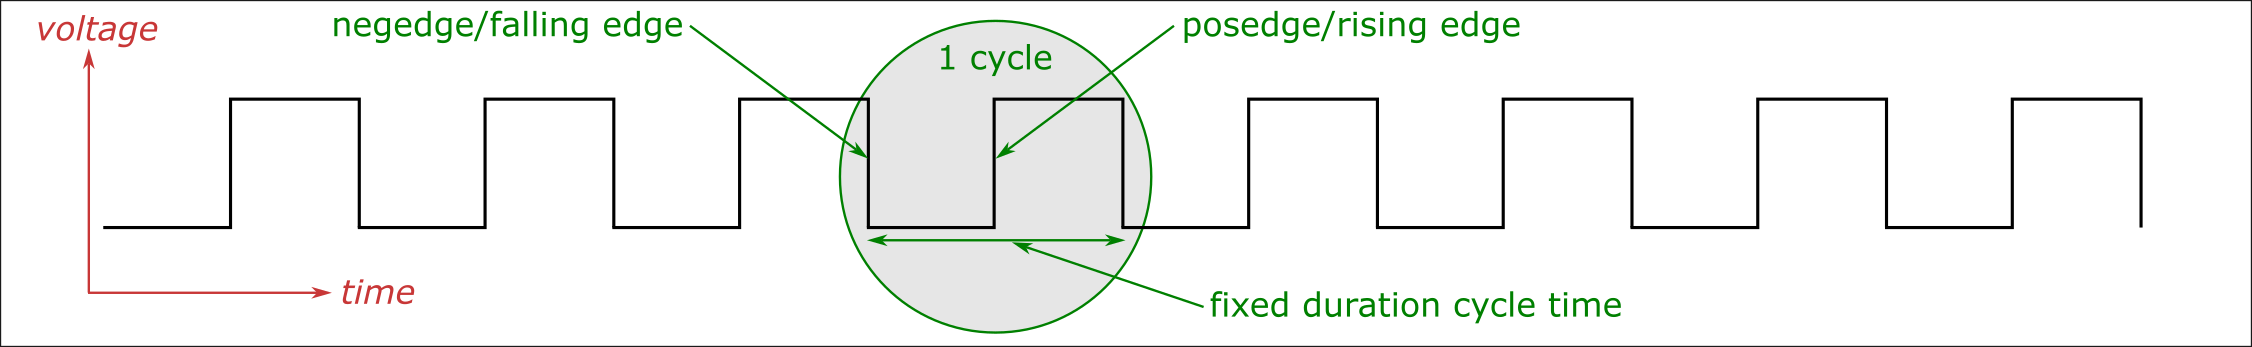
\includegraphics[width=0.6\textwidth]{Fig_Clock}}
\end{center}

\vspace{1ex}

Any value that must be visible from one clock to the next must be
stored in a \emph{state element} (a component that can ``remember''
values, {\ie} has \emph{state}, like a register, FIFOF, buffer,
memory, ...).

\end{frame}

% ================================================================

\begin{frame}
\frametitle{General structure and operation of digital circuits}

\footnotesize

\begin{center}
\frame{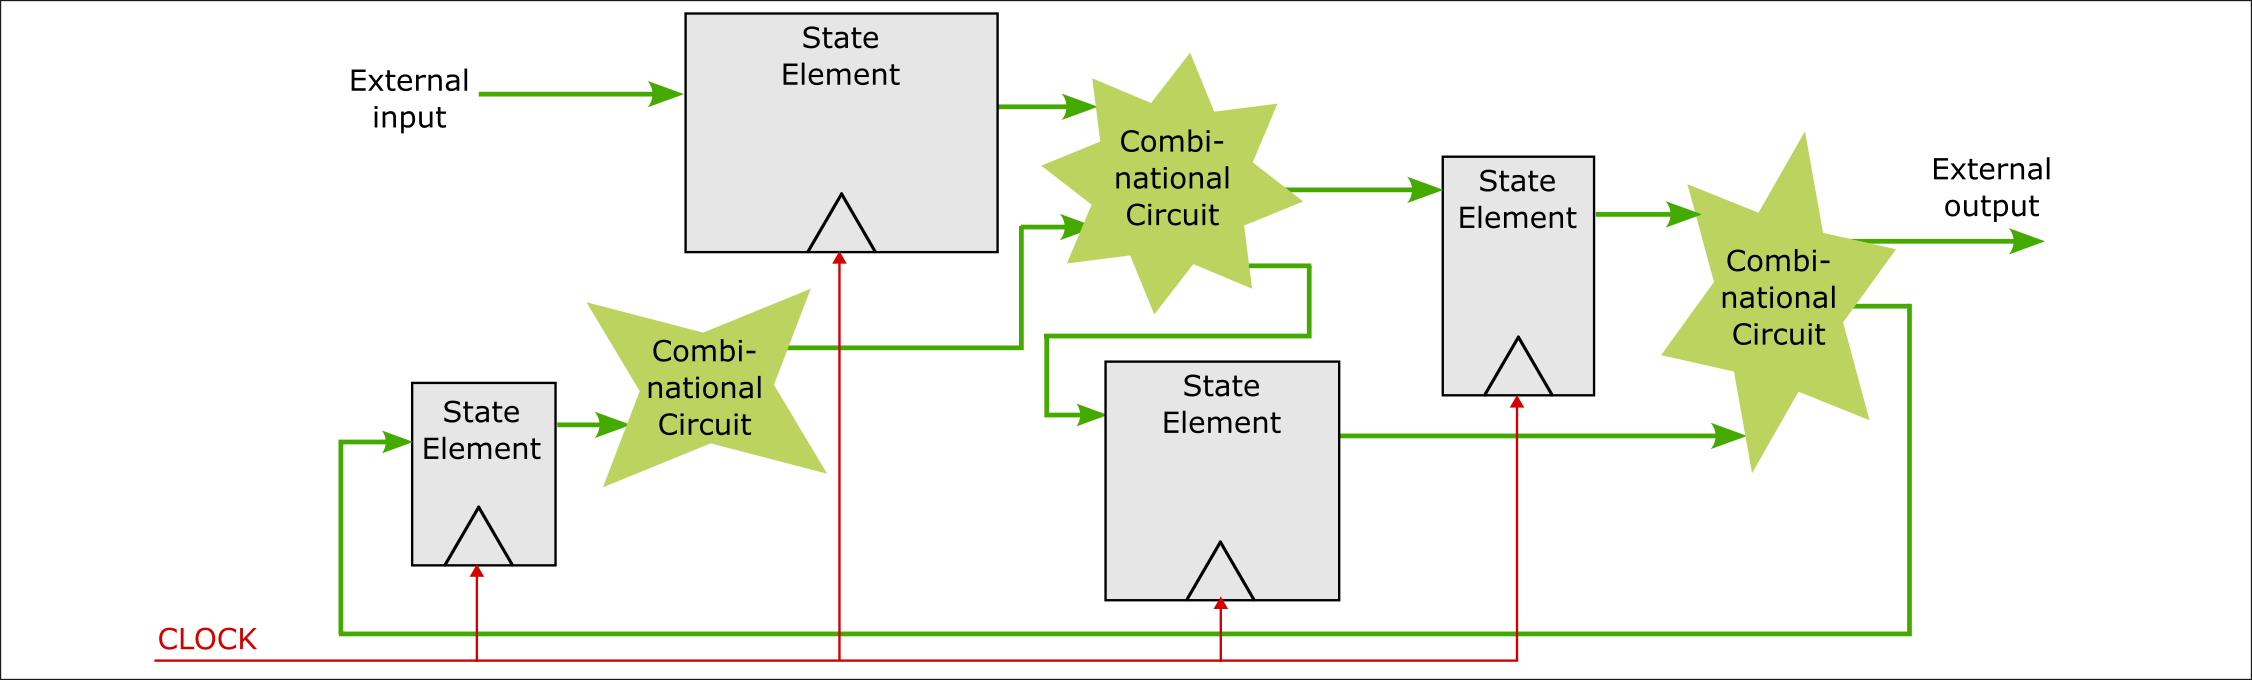
\includegraphics[width=0.8\textwidth]{Fig_BSV_Digital_Circuits}}
\end{center}

Digital circuits are composed of \emph{state elements} and
\emph{combinational circuits} connecting outputs of state elements to
inputs of state elements.  State elements are \emph{storage} elements.
Combinational circuits are \emph{acyclic} networks of \emph{logic
gates} (AND, OR, NOT, ...).  Any digital circuit repeatedly performs
the following:

\begin{itemize}

\item After each ``posedge'' (positive edge of a clock), the
      combinational circuits compute new inputs for all state
      elements, based on the current values in state elements

\item At the next posedge, these new input values are stored into the
      state elements.

\end{itemize}

\end{frame}

% ================================================================

\begin{frame}
\frametitle{General operation of digital circuits; notes and caveats}

\footnotesize

\begin{itemize}
 \item Nowadays, clock cycle times/periods are typically measured in
       nanoseconds. \\
       For example, a 100 MHz clock has a 10ns cycle time.

 \item Physics and circuit silicon technology dictates how long an
       electrical signal takes to propagate from the output of a state
       element and through a combinational circuit before it arrives
       at the input of a state element.  The clock period needs to be
       greater than this.

       In the \emph{digital abstraction} we assume this condition is
       met, and we ``idealize'' wire and combinational circuit delays
       as taking zero time.

\end{itemize}

\PAUSE{\vspace{2ex}}

\begin{itemize}

 \item Advanced digital ciruits may have multiple clocks driving
       different parts of the circuit.

 \item Advanced digital ciruits may vary the clock speed dynamically,
       to match power consumption to current performance demands
       (higher speeds $\Rightarrow$ more power consumption).

 \item Some digital ciruits use the negative edge (``negedge'') of the
       clock insted of the posedge.

 \item Advanced digital ciruits may use both the posedge and the
       negedge of the clock.

\end{itemize}

\end{frame}

% ================================================================

\begin{frame}
\frametitle{Computer Memories}

\footnotesize

\begin{center}
\frame{\includegraphics[width=0.9\textwidth]{Fig_BSV_Split_Phase_Mem}}
\end{center}

\vspace*{2ex}

A computer memory is a packaged device providing \emph{random access}
to a sequence of locations:

\begin{itemize}

 \item To read memory, we present a \emph{read request} at its inputs,
       with an \emph{address}; \\
       the memory provides a \emph{read response} at its outputs,
       containing the addressed data.

 \PAUSE{}

 \item To write memory, we present a \emph{write request} at its
       inputs, with an address and data; \\
       the memory provides a \emph{write response} at its outputs,
       containing an ``ok'' status.

\end{itemize}

\end{frame}

% ================================================================

\begin{frame}
\frametitle{Kinds of Computer Memory}

\footnotesize

\begin{center}
\frame{\includegraphics[width=0.9\textwidth]{Fig_BSV_Split_Phase_Mem}}
\end{center}

{\footnotesize
\begin{itemize}
 \item SRAMs (Static Random Access Memories)
       \begin{itemize}\footnotesize
        \item Typically from a few kilobytes to a few megabytes
	\item Faster than DRAM
	\item More power-consumption than DRAM
	\item Often used for ``caches'' close to the CPU.
       \end{itemize}

 \item DRAMs (Dynamic Random Access Memories)
       \begin{itemize}\footnotesize
        \item Typically from a few megabytes to gigabytes
	\item Slower than SRAM
	\item Less power-consumption than SRAM
	\item Often used for caches and ``main memory'' further away from the CPU.
       \end{itemize}
\end{itemize}}

\end{frame}

% ================================================================

\begin{frame}
\frametitle{Split-phase Memory Access}

\footnotesize

\begin{center}
\frame{\includegraphics[width=0.9\textwidth]{Fig_BSV_Split_Phase_Mem}}
\end{center}

\vspace*{1ex}

Typically (for any memory larger than a few kilobytes), the response
is available \emph{one or more clocks after} the inputs were
presented.  We also say that memory accesses are
\alert{split-phase}---requiring temporally separated request-production
and response-consumption.

\vspace*{1ex}

\PAUSE{\vspace{1ex}}

The delay from when the CPU issues a request until when it can collect
the response is called \emph{memory latency} (units: clock cycles,
nanoseconds).

\end{frame}

% ================================================================

\begin{frame}
\frametitle{Pipelined Memory Access}

\footnotesize

\begin{center}
\frame{\includegraphics[width=0.9\textwidth]{Fig_BSV_Split_Phase_Mem}}
\end{center}

\vspace*{1ex}

The CPU $\Rightarrow$ memory $\Rightarrow$ CPU path is often pipelined
and behaves like a queue:

{\footnotesize
\begin{itemize}

 \item The CPU can pump in requests towards memory without waiting for responses.

 \item Concurrently, another part of the CPU can pump out responses from memory.
\end{itemize}}

\PAUSE{\vspace{1ex}}

The rate at which the CPU can pump requests is called \emph{memory
bandwidth} (units: transactions/second, requests/second, bytes/second).

\vspace*{1ex}

\PAUSE{\vspace{1ex}}

Latency and bandwidth can vary (may depend on size of memory request,
cache misses, virtual memory page faults, cache coherence traffic,
...).

\end{frame}

% ================================================================

\begin{frame}[fragile]
\frametitle{Memory Hierarchies}

\footnotesize

Most modern computers have one or more levels of \emph{cache} memories
between the CPU and main memory.

\vspace{1ex}

\begin{center}
 \frame{\includegraphics[width=0.8\textwidth]{Fig_Mem_Hierarchy}}
\end{center}

\begin{itemize}

 \item Each level typically holds a subset of memory locations held at
       the next level.

 \PAUSE{}

 \item At any level L$_j$, if a request from level L$_{j-1}$ is for
       one of these cached locations, it can respond immediately
       (cache ``hit'').  Otherwise it is a ``miss'', and the memory
       location needs to be fetched (``refill'') from level L$_{j+1}$
       (to make room for this, it may have to write back some other
       cached location to level L$_{j+1}$ (``writeback'')).

 \PAUSE{}

 \item Each level independently transacts with the next level
       (although, usually, a miss at one level will trigger writeback
       and refill transactions with the next level).  These are
       usually also split-phase, and may or may not be pipelined.

\end{itemize}

\end{frame}

% ================================================================

% -*- mode: fundamental -*-

% Slides accompanying "Learn RISC-V CPU Implementation and BSV" book
% Copyright (c) 2024 Rishiyur S. Nikhil, All Rights Reserved

% This is a postamble shared by all the slide decks

% ================================================================

\begin{frame}

\begin{center}
  {\LARGE End}
\end{center}

\end{frame}

% ================================================================


% ****************************************************************

\end{document}
